\chapter{Data analysis and Event reconstruction}\label{section:Reconstruction}


\section{Data analysis}\label{sec:Data analysis}
\subsection{Event selection}\label{subsec:Event selection}
The top all hadronic decay channel has 2 b-jets and 4 quark jets, all of them in our configuration are not in the boosted region. Follow the event selection used in the reference\cite{Mccarthy:2015ucy},  we apply a event selection that an event should at least exists \textbf{2 b-jets} and \textbf{4 quark jets} satisfied $p_{T}$ larger than \textbf{25 GeV} and $|\eta|$ less than \textbf{2.5}. A cutflow table and figure can help us to understand how many events are killed by the selections. We may apply 5 cuts and see the evolution of survived event numbers. The rule of cuts is shown in Table \ref{table:cuts}, and the cutflow is shown in Figure \ref{fig:cutflow}. As the result, we found around 18\~20\% of events will survive after the event selection. 

\begin{center}
	\begin{table}[h]
		\begin{tabular}{p{0.1\textwidth} c c c }
			\cline{1-3}
			\#Cut    & Number of b-jets & Number of quark jets  \\
			\hline
			C1      &   0  & 4    \\
			C2      &   0  & 5    \\
			C3      &   0  & 6    \\
			C4      &   1  & 6    \\
			C5      &   2  & 6    \\
			\hline
		\end{tabular}
		\caption{Rule of cuts. All the cuts require a kinematic limitation that $p_{T} > 25$ GeV and $|\eta|<2.5$.}
		\label{table:cuts}
	\end{table}
\end{center}

\begin{figure}[!h]
	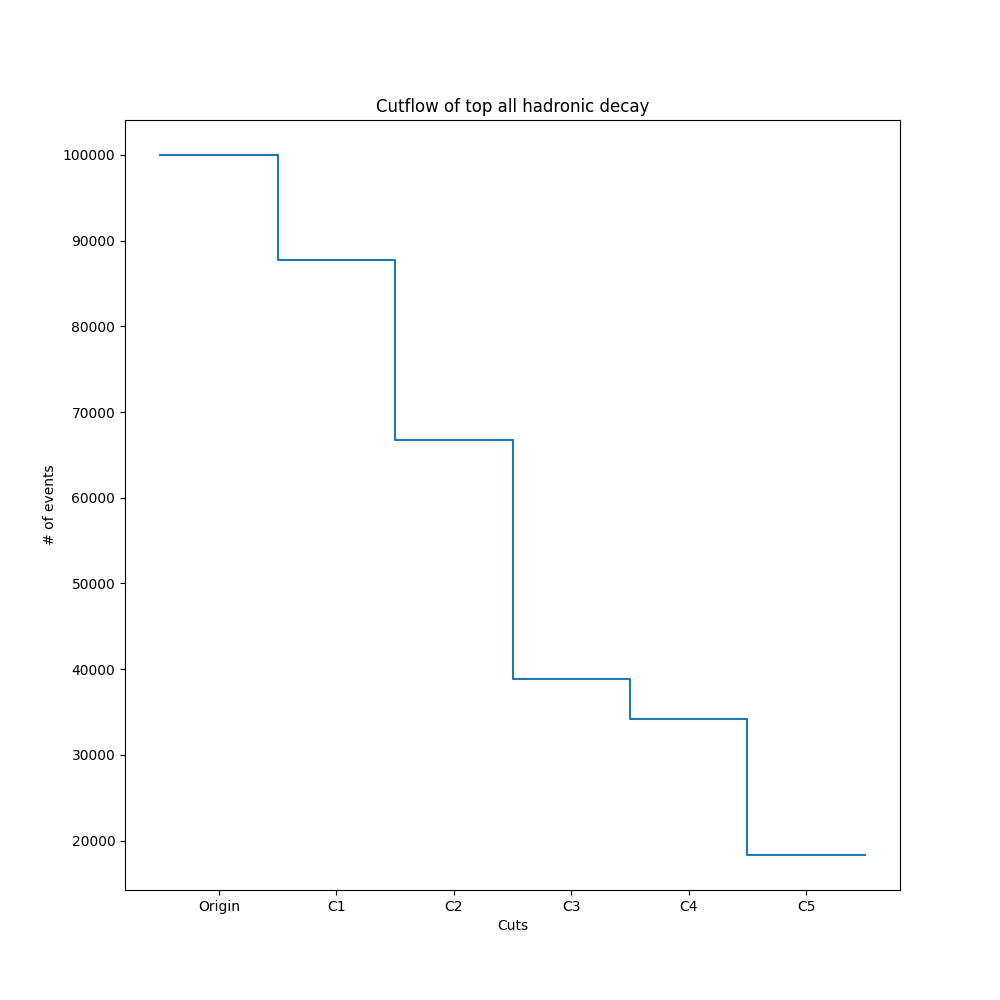
\includegraphics[width=0.8\linewidth, height=7cm,keepaspectratio=true]{Figures/ttbar_cutflow.png}
	\caption{Cutflow of all hadronic top decay.}
	\label{fig:cutflow}
\end{figure}
\begin{figure}[H]
	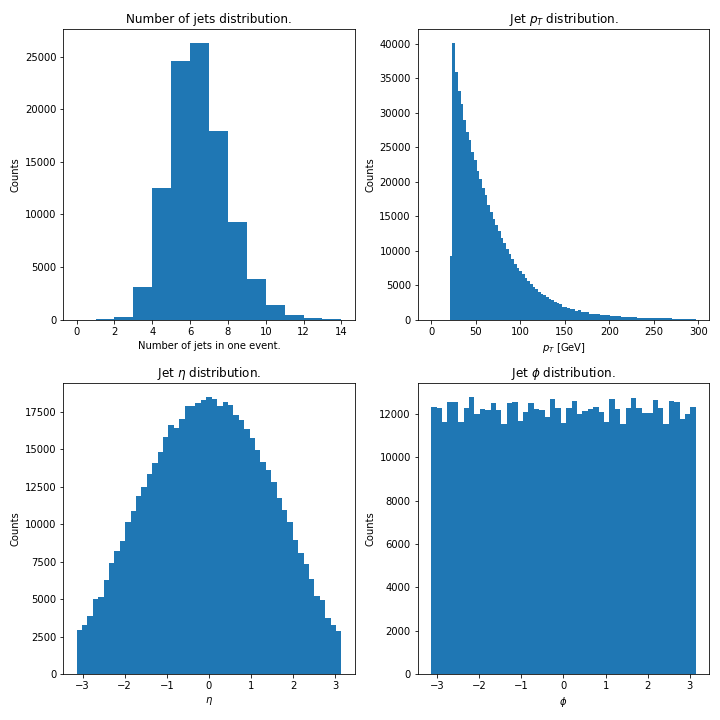
\includegraphics[width=0.8\linewidth, height=8cm,keepaspectratio=true]{Figures/ttbar_kinematic_dist.png}
	\caption{Demonstration of distributions.}
	\label{fig:kinematic dist}
\end{figure}
\newpage

\subsection{Truth matching}\label{subsec:Truth matching}
The \textbf{truth matching}, which is also called \textbf{$\Delta$R matching},  is to match the detector simulation(i.e. jet information generate by Delphes) data to truth record(i.e. Parton level information).  To calculate the $\Delta R$ value, we will find the daughters of top quarks, W boson, and b quark. After the daughters of top quarks are found, we will find the daughters of W bosons. Finally, we will get six partons that come from the decay of top quark pairs. These six partons can match the jets identically by considering their distances. The formula of calculating $\Delta R$ is:
\\
\begin{equation}
	\Delta R = \sqrt{\Delta\eta^{2} + \Delta\phi^{2}}
\end{equation}
By using the kinematic properties provide in parton level and detector simulation information, we can calculate the $\Delta R$ value between each parton and jets. Using the result of the calculation, we may assign each parton to a specific jet. 
\\
\subsection{Custom barcode system}\label{subsec:barcode}
To specify the relation between each parton, and the relation between mothers and daughters, we design a barcode system that helps us to declare the relationship.
\begin{figure}[H]
	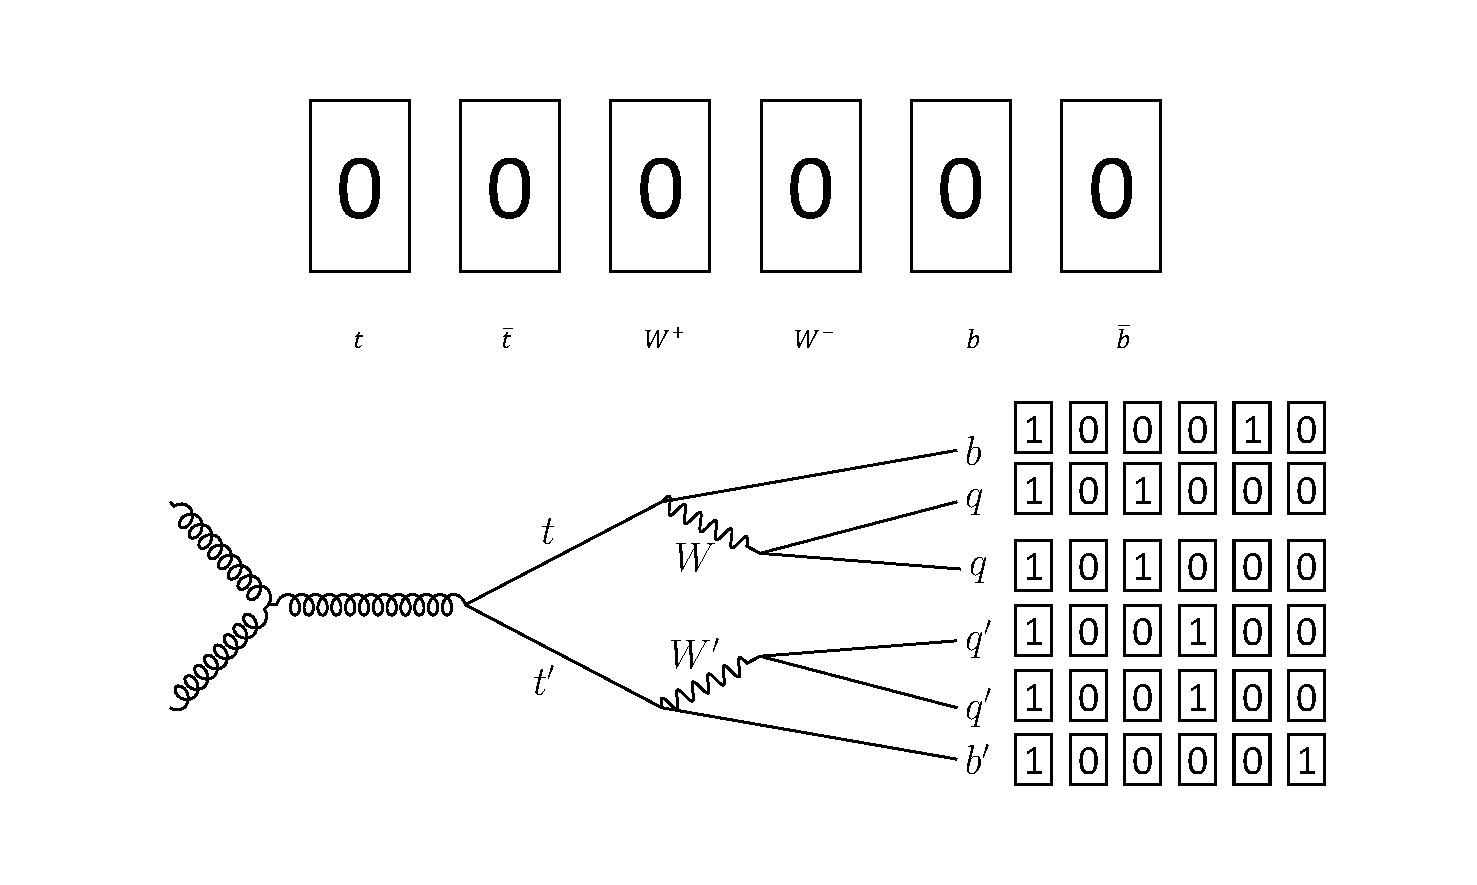
\includegraphics[width=0.8\linewidth]{Figures/barcode.pdf}
	\caption{Design of barcode.}
	\label{fig:barcode}
\end{figure}
\newpage
In Figure \ref{fig:barcode}, we define a six-digit barcode, the first two digits are to show which top quark is the mother of this parton, the last four digits of the sequence is to declare which daughter of the top quark is the mother of parton. In case, we can use this barcode system to break six parton(jet) candidates into two subsets which contains 3 elements. The benefit of using this barcode system is not only can specify the relation without losing the information, but also provide a permutation relationship to our network. We will discuss this in the following section.

\section{Event reconstruction}\label{sec:Event reconstruction}

\subsection{$\chi^{2}$ minimization method}\label{subsec:chi-square}

The $\chi^{2}$ minimization method is a traditional method to reconstruct an event. For an event that exists 6 jets, it has about $6!/(2\times2\times2)=90$ possible combinations. It is obvious that the number of probable combinations is propotional to the number of exist jets in an event. The $\chi^{2}$ minimization method will calculate all the candidates and try to find the candidate which has the smallest $\chi^{2}$ value. This method base on the masses of W boson and top quark(or you may consider the difference of the top masses reconstructed by two subsets.). The equation of $\chi^{2}$ minimization in this model is:

\begin{equation}
	\chi^{2} = \frac{(m_{bqq'} - m_{\bar{b}q''q'''})^{2}}{\sigma^{2}_{\Delta_{m_{bqq'}}}}  + \frac{(m_{qq'} - m_{W})^{2}}{\sigma^{2}_{W}} + \frac{(m _{q''q'''} - m_{W})^{2}}{\sigma^{2}_{W}}
\end{equation} 


\subsection{Machine Learning Approach}\label{subsec:ML approach}

For a machine learning model, equivariance and invariance are the important properties that may effect the performance of the model. Such as the computer vision problem, the object should be invariant under translation to prevnet affect the prediction. Convolutional Neural Network(CNN) can produce object recongition outcome that are invariance under translations. The properties of invariance can be generalized to another geometry sturcture, e.g. manifolds and groups. In all hadronic top decay, we have two subsets with the same elements $(b, q, q')$ and $(\bar{b}, q'', q''')$. These subsets should remain invariant under permutations of the input jets order. 
\\
Attention mechanism is a architecture that allow the network to propagate the information selectively by using a "mask". By the implement of mask, the neural network can learn from partial information and update the parameters with selected information, and allow network to infer the relationships between different elements in a sequence.
\\
By the invariant feature of attention architecture, rearranging the element in a sequences leave the attention weight unchange. We may use this permutation symmetry presnet the attention-based model can handle the reconstruction of all hadronic top decay process effiently. In case, the network output of the all hadronic top decay process should identify two distint interchangeable subsets, each  contains interchangeable $qq$ pair. This invariant property on the output is the unique feature of our dataset and the model should take into account. 


